\section{Discussion} \label{sec:discussion}

\subsection{No external forces}
\label{sec:discussion:no}

In the beginning of the experiment, no external forces were being exerted on the gyroscope, and the motion of its rotor axis was observed upon gentle tilting or rotation of the base\footnote{Tilting or rotating in such a way that the rotor axis does not experience any external torque.}. The rotor axis maintained its spatial orientation with respect to an inertial frame (e.g., the table's frame of reference). This resistivity is based on the conservation of angular momentum ($\vec{L} = \mathbf{I}\vec{\omega} = const$) when no external torques are applied. Because the angular momentum vector remained constant in orientation and magnitude, and $\hat{x}_{3}$ rotor axis is the principal axis of the gyroscope, its spinning angular velocity ($\boldsymbol\omega_{3}$) is aligned with the angular momentum. Thus, the spinning angular velocity ($\boldsymbol\omega_{3}$) also maintains its orientation and magnitude.

\begin{figure}[H]
  \centering
  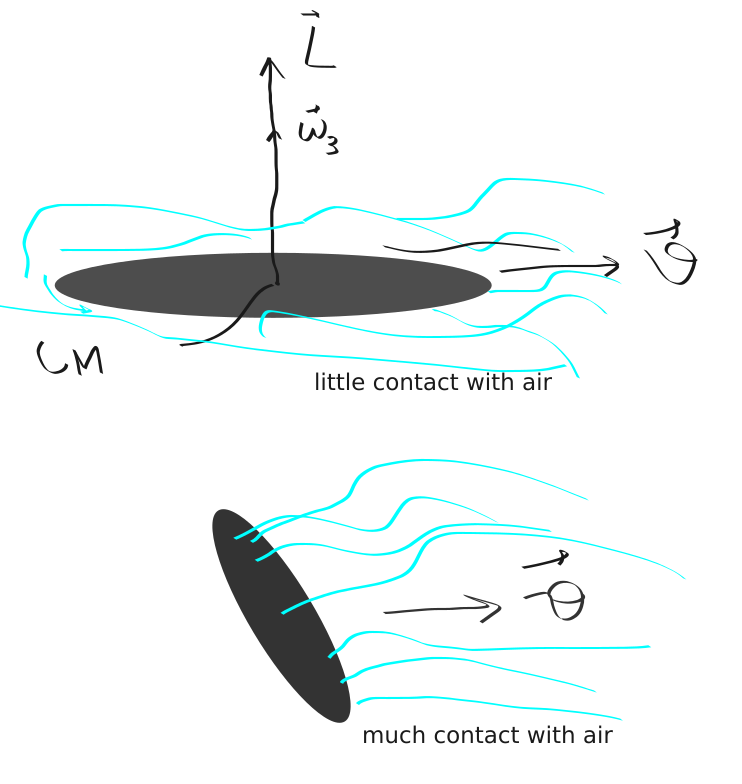
\includegraphics[width=\columnwidth]{gyroscope/images/thin}
  \caption{Aerodynamics of a thin object }
  \label{fig:discussion:thin}
\end{figure}

Notably, this phenomenon explains why it is possible to throw a regularly shaped, thin object (e.g., a frisbee or discus) over longer distances if it is given a spin rather than if it is not rotating. Achieving long-distance transportation requires stability and sufficient airodynamic properties to resist air resistivity. If the object is given a spin around its center of mass as shown in figure \ref{fig:discussion:thin}, its angular momentum is conserved during flight in the absence of external torques. This conservation counteracts air's random force fluctuations on the object's surface, maintaining its aerodynamic orientation (i.e.,the thin face aligned in the direction of motion). Consequently, this object will travel over longer distances. Conversely, if no spinning is applied, random force fluctuations in air on the object surface will deorient and destabilize the object, effectively reducing its aerodynamic properties. Thus, this object will not travel as far due to higher air resistivity. 

\subsection{Improvements} \label{sec:discussion:improvements}

An insufficient number of processed precession frequencies ($\Omega$) and corresponding spinning periods ($T_{3}$) significantly affected the error in the calculation of the slope (TODO: which slope). Additionally, certain aspects of the gyroscope setup introduced deviation from the theoreical ideal case:

1. The vertical axis of the gyroscope was not perfectly aligned, resulting in a slight tilt.

2. During the gyroscope's motion, both the counterweights and torque-introducing weights experienced small linear displacement relative to the roto's axis accelerating frame of reference.

3. The initial spinning frequency ($\omega_{3}$) and the attachment of counterweights were set and adjusted by eye, which inherently introduced human error. This error was big for the initial spinning frequencies ($\omega_{3}$).

In order to calculate the precession period $T_{p_{calculated}}$ accurately, many precession frequency samples were required for each measurement\footnote{Each measurement has the same magnitude of the initial spinning angular frequency ($\omega_{3}$) and the applied torque (mass-lever-arm couple)}. However, since the initial spinning angular frequency was imparted by manually pulling a string wrapped around the rotor's reel, it was impossible to ensure consistency in torque and spinning frequency for each sample per measurement. This introduced significant uncertainty in $\omega_{3}$ accross measurements.

Moreover, pure precession of the gyroscope was not always achieved. In many instances, nutation was observed during the motion. The following actions were taken in response to this:

1. If nutation diminished over time, the dataset was trimmed to retain only the segment coressponding to pure precession.

2. If nutation persisted, mean precession frequency was estimated (see section \ref{sec:theory:nutation}).

In either case, nutation established noise in data, leading to bigger uncertainty in the precession frequencies ($\Omega$).

Finally, the spinning period ($T_{3}$) was calculated by manually estimating the time needed to make a full revolution (see \ref{sec:methods}) and evaluating the mean and the mean squared error. This manual calculation brought in a big error in the spinning period ($T_{3}$).

To improve the accuracy of the slope and strengthen the foundation for the research question of this lab report, the following steps are recommended. First, a digital motor controlled by software can be used to launch and maintain the rotor. This would ensure a precise, constant, and controlled initial spinning angular velocities for each sample per every measurement. Besides, videos of the spinning of the rotor can be fed into a neural network capable of feature extracting (e.g., see \cite{2}). Neural network extracts the spinning period ($T_{3}$) with a much higher accuracy. Alternatively, a separate sensor can be placed in the precessing frame of reference that would measure the spinning period during the course of the sample's motion. Lastly, counterweights and torque-introducing weights should be set in-place using, for instance, nails protruding through the rotory axis. The locations for all weights should be estimated using computer techniques.   
